\chapter{Perl Summary}
\label{chap:chapterab}
\minitoc

This appendix summarizes those parts of the Perl programming language that will be most useful to you as you read this book. It is not a comprehensive summary of the Perl language. Remember that Perl is designed so that you don't need to know everything in order to use it. Source material for this appendix came from \textit{Programming Perl, Third Edition} (O'Reilly \& Associates).

\section{Command Interpretation}
The Perl programs in this book start with the line:

\begin{lstlisting}
#!/usr/bin/perl -w
\end{lstlisting}

On Unix (or Linux) systems, the first line of a file can include the name of a program and some flags, which are optional. The line must start with \verb|#!|, followed by the full pathname of the program (in our case, the Perl interpreter), followed optionally by a single group of one or more flags.

If the Perl program file was called \textit{myprogram}, and had executable permissions, you can type \verb|myprogram| (or possibly \verb|./myprogram|, or the full or relative pathname for the program) to start the program running.

The Unix operating system starts the program specified in the command interpretation line and gives it as input the rest of the file after the first line. So, in this case, it starts the Perl interpreter and gives it the program in the file to run.

This is just a shortcut for typing:

\begin{lstlisting}
/usr/bin/perl -w myprogram 
\end{lstlisting}

at the command line.

\section{Comments}
A comment begins with a \# sign and continues from there to the end of the same line. It is ignored by the Perl interpreter and is only there for programmers to read. A comment can include any text.

\section{Scalar Values and Scalar Variables}
A scalar value is a single item of data, like a string or a number.

\subsection{Strings}
Strings are scalar values and are written as text enclosed within single quotes, like so:

\begin{lstlisting}
'This is a string in single quotes.'
\end{lstlisting}

or double quotes, such as:

\begin{lstlisting}
"This is a string in double quotes."
\end{lstlisting}

A single-quoted string prints out exactly as written. With double quotes, you can include a variable in the string, and its value will be inserted or "interpolated." You can also include commands such as \verb|\n| to represent a newline (see \autoref{tab:tablea.b3}):

\begin{lstlisting}
$aside = '(or so they say)';
$declaration = "Misery\n $aside \nloves company.";
print $declaration;
\end{lstlisting}

This snippet prints out:

\begin{lstlisting}
Misery 
 (or so they say) 
loves company.
\end{lstlisting}

\subsection{Numbers}
Numbers are scalar values that can be:

\begin{itemize}
  \item Integers:\\ \verb|3|\\ \verb|-4|\\ \verb|0|
  \item Floating-point (decimal):\\ \verb|4.5326|
  \item Scientific (exponential) notation ($3.13 \times 10^{23}$ or 313000000000000000000000):\\ \verb|3.13E23|
  \item Hexadecimal (base 16):\\ \verb|Ox12bc3|
  \item Octal (base 8):\\ \verb|O5777|
  \item Binary (base 2):\\ \verb|0b10101011|
\end{itemize}

Complex (or imaginary) numbers, such as \verb|3 + i|, and fractions (or ratios, or rational numbers), such as \verb|1/3|, can be a little tricky. Perl can handle fractions but converts them internally to floating-point numbers, which can make certain operations go wrong (Perl is not alone among computer languages in this regard.):

\begin{lstlisting}
if ( 10/3  == ( (1/3) * 10  ) {
  print "Success!";
}else {
  print "Failure!";
}
\end{lstlisting}

This prints:

\begin{lstlisting}
Failure!
\end{lstlisting}

To properly handle rational arithmetic with fractions, complex numbers, or many other mathematical constructs, there are mathematics modules available, which aren't covered here.

\subsection{Scalar Variables}
Scalar values can be stored in scalar variables. A scalar variable is indicated with a \verb|$| before the variable's name. The name begins with a letter or underscore and can have any number of letters, underscores, or digits. A digit, however, can't be the first character in a variable name. Here are some examples of legal names of scalar variables:

\begin{lstlisting}
$Var
$var_1
\end{lstlisting}

Here are some improper names for scalar variables:

\begin{lstlisting}
$1var
$var!iable
\end{lstlisting}

Names are case sensitive: \verb|$dna| is different from \verb|$DNA|.

These rules for making proper variable names (apart from the beginning \verb|$|) also hold for the names of array and hash variables and for subroutine names.

A scalar variable may hold any type of scalar value mentioned previously, such as strings or the different types of numbers.

\section{Assignment}
Scalar variables are assigned scalar values with an assignment statement. For instance:

\begin{lstlisting}
$thousand = 1000;
\end{lstlisting}

assigns the integer 1,000, a scalar value, to the scalar variable \verb|$thousand|.

The assignment statement looks like an equal sign from elementary mathematics, but its meaning is different. The assignment statement is an instruction, not an assertion. It doesn't mean "\verb|$thousand| equals 1,000." It means "store the scalar value 1,000 into the scalar variable \verb|$thousand|". However, after the statement, the value of the scalar variable \verb|$thousand| is, indeed, equal to 1,000.

You can assign values to several scalar variables by surrounding variables and values in parentheses and separating them by commas, thus making lists:

\begin{lstlisting}
($one, $two, $three) = ( 1, 2, 3 );
\end{lstlisting}

There are several assignment operators besides \verb|=| that are shorthand for longer expressions. For instance, \verb|$a += $b| is equivalent to \verb|$a = $a + $b|. \autoref{tab:tablea.b1} is a complete list (it includes several operators that aren't covered in this book).

\begin{table}[!htbp]
  \begin{center}
  \caption{Assignment operator shorthands}
  \label{tab:tablea.b1}
  %\begin{tabu}{X[1,c]X[2,l]}
    \begin{tabu*} to 0.7\linewidth {X[1,c,m]X[3,l,m]}
    \toprule
    Example of operator & Equivalent\\
    \midrule
    \verb|$a += $b| & \verb|$a = $a + $b| (addition)\\
    \verb|$a -= $b| & \verb|$a = $a - $b| (subtraction)\\
    \verb|$a *= $b| & \verb|$a = $a * $b| (multiplication)\\
    \verb|$a /= $b| & \verb|$a = $a / $b| (division)\\
    \verb|$a **= $b| & \verb|$a = $a ** $b| (exponentiation)\\
    \verb|$a |\%\verb|= $b| & \verb|$a = $a |\%\verb| $b| (remainder of \verb|$a/$b|)\\
    \verb|$a x= $b| & \verb|$a = $a x $b| (string \verb|$a| repeated \verb|$b| times)\\
    \verb|$a &= $b| & \verb|$a = $a & $b| (bitwise AND)\\
    \verb+$a |= $b+ & \verb+$a = $a | $b+ (bitwise OR)\\
    \verb|$a ^= $b| & \verb|$a = $a ^ $b| (bitwise XOR)\\
    \verb|$a >>= $b| & \verb|$a = $a >> $b| (\verb|$a| shift \verb|$b| bits)\\
    \verb|$a <<= $b| & \verb|$a = $a << $b| (\verb|$a| shift \verb|$b| bits to left)\\
    \verb|$a &&= $b| & \verb|$a = $a && $b| (logical AND)\\
    \verb+$a ||= $b+ & \verb+$a = $a || $b+ (logical OR)\\
    \verb|$a .= $b| & \verb|$a = $a . $b| (append string \verb|$b| to \verb|$a|)\\
    \bottomrule
    \end{tabu*}
  \end{center}
\end{table}

\section{Statements and Blocks}
Programs are composed of statements often grouped together into blocks.

A statement ends with a semicolon (;), which is optional for the last statement in a block.

A block is one or more statements usually surrounded by curly braces; here's an example:

\begin{lstlisting}
{
  $thousand = 1000;
  print $thousand;
}
\end{lstlisting}

Blocks may stand by themselves but are often associated with such constructs as loops or \verb|if| statements.

\section{Arrays}
Arrays are ordered collections of zero or more scalar values, indexed by position. An array variable begins with the at sign \verb|@| followed by a legal variable name. For instance, here are two possible array variable names:

\begin{lstlisting}
@array1
@dna_fragments
\end{lstlisting}

You can assign scalar values to an array by placing the scalar values in a list, separated by commas and surrounded by a pair of parentheses. For instance, you can assign an array the empty list:

\begin{lstlisting}
@array = ( );
\end{lstlisting}

or one or more scalar values:

\begin{lstlisting}
@dna_fragments = ('ACGT', $fragment2, 'GGCGGA');
\end{lstlisting}

Notice that it's okay to specify a scalar variable such as \verb|$fragment2| in a list. Its current value, not the variable name, is placed into the array.

The individual scalar values of an array (the elements) are indexed by their position in the array. The index numbers begin at 0. You can specify the individual elements of an array by preceding the array name by a \verb|$| and following it with the index number of the element within square brackets \verb|[ ]|, like so:

\begin{lstlisting}
$dna_fragments[2]
\end{lstlisting}

This equals the value of '\verb|GGCGGA|', given the values previously set for this array. Notice that the array has three scalar values, indexed by numbers 0, 1, and 2. The third and last element is indexed 2, one less than the total number of elements 3, because the first element is indexed number 0.

You can make a copy of an array using an assignment operator \verb|=|, as in this example that makes a copy \verb|@output| of an existing array \verb|@input|: 

\begin{lstlisting}
@output = @input;
\end{lstlisting}

If you evaluate an array in scalar context, the value is the number of elements in the array. So if array \verb|@input| has five elements, the following example assigns the value 5 to \verb|$count|:

\begin{lstlisting}
$count = @input;
\end{lstlisting}

\autoref{fig:figurea.b1} shows an array \verb|@myarray| with three elements, which demonstrates the ordered nature of an array; by which each element appears, and can be found by its position in the array.

\begin{figure}
  \centering
  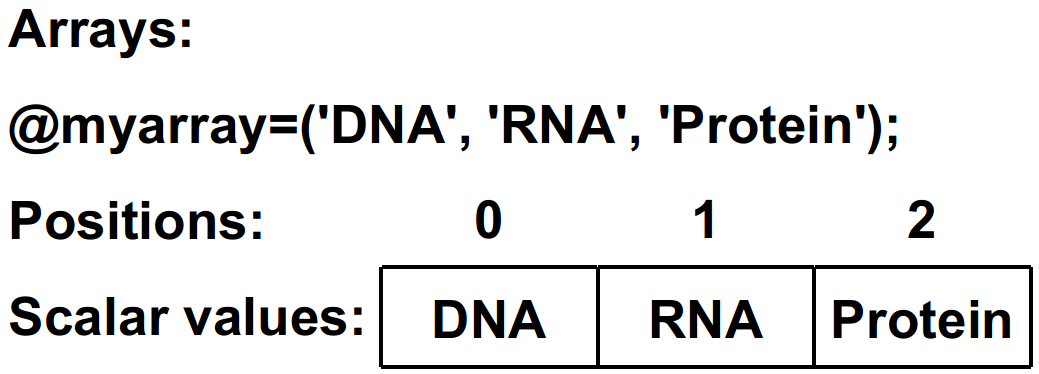
\includegraphics[width=0.5\textwidth]{figurea_b1.png}
  \caption{Schematic of an array}
  \label{fig:figurea.b1}
 \end{figure}{}

\section{Hashes}
A hash (also called an associative array) is a collection of zero or more pairs of scalar values, called keys and values. The values are indexed by the keys. An hash variable begins with the percent sign \verb|%| followed by a legal variable name. For instance, possible hash variable names are:

\begin{lstlisting}
%hash1
%genes_by_name
\end{lstlisting}

You can assign a value to a key with a simple assignment statement. For example, say you have a hash called \verb|%baseball_stadiums| and a key \verb|Phillies| to which you want to assign the value \verb|Veterans Stadium|. This statement accomplishes the assignment:

\begin{lstlisting}
$baseball_stadiums{'Phillies'} = 'Veterans Stadium';
\end{lstlisting}

Note that a single hash value is referenced by a \verb|$| instead of a \verb|%| at the beginning of the hash name; this is similar to the way you reference individual array values by using a \verb|$| instead of a \verb|@|.

You can assign several keys and values to a hash by placing their scalar values in a list, separated by commas and surrounded by a pair of parentheses. Each successive pair of scalars becomes a key and a value in the hash. For instance, you can assign a hash the empty list:

\begin{lstlisting}
%hash = ( );
\end{lstlisting}

You can also assign one or more scalar key-value pairs:

\begin{lstlisting}
%genes_by_name = ('gene1', 'AACCCGGTTGGTT', 'gene2', 'CCTTTCGGAAGGTC');
\end{lstlisting}

There is an another way to do the same thing, which makes the key-value pairs more readily apparent. This accomplishes the same thing as the preceding example:

\begin{lstlisting}
%genes_by_name = (
  'gene1' => 'AACCCGGTTGGTT',
  'gene2' => 'CCTTTCGGAAGGTC'
);
\end{lstlisting}

To get the value associated with a particular key, precede the hash name with a \verb|$| and follow it with a pair of curly braces \verb|{ }| containing the scalar value of the key:

\begin{lstlisting}
$genes_by_name{'gene1'}
\end{lstlisting}

This returns the value '\verb|AACCCGGTTGGTT|', given the value previously assigned to the key '\verb|gene1|' in the hash \verb|%genes_by_name|. \autoref{fig:figurea.b2} shows a hash with three keys.

\begin{figure}
  \centering
  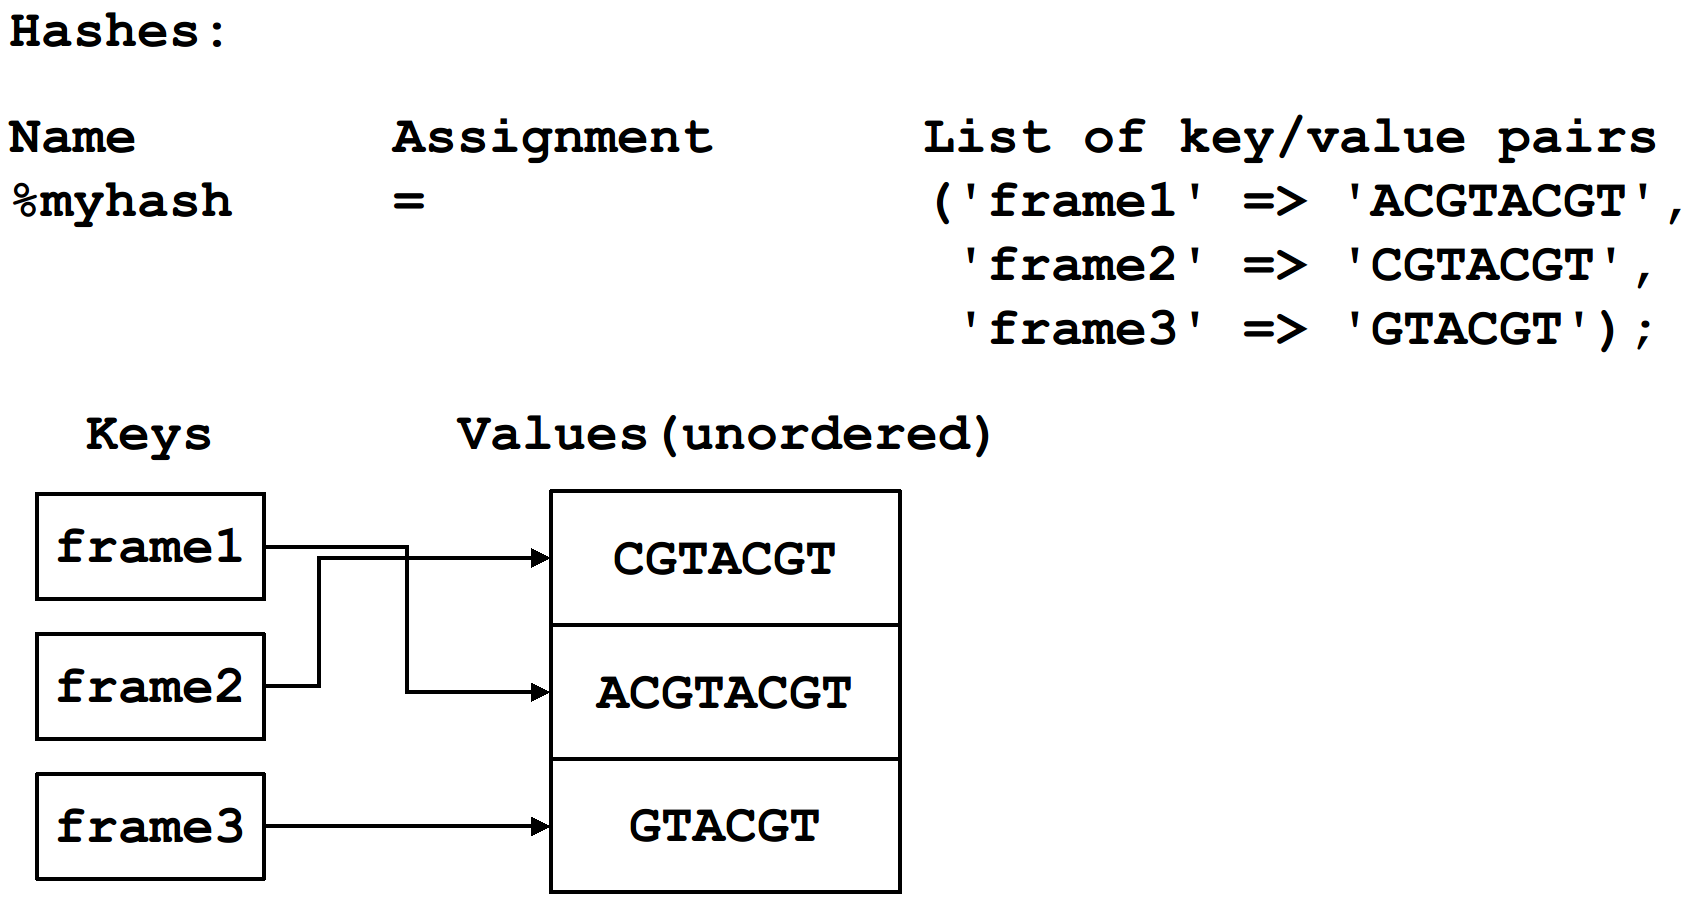
\includegraphics[width=0.7\textwidth]{figurea_b2.png}
  \caption{Schematic of a hash}
  \label{fig:figurea.b2}
 \end{figure}{}

\section{Operators}
Operators are functions that represent basic operations on values: addition, subtraction, etc. They are frequently used and are core parts of the Perl programming language. They are really just functions that take arguments. For instance, \verb|+| is the operator that adds two numbers, like so:

\begin{lstlisting}
3 + 4;
\end{lstlisting}

Operators typically have one, two, or three operands; in the example just given, there are two operands \verb|3| and \verb|4|.

Operators can appear before, between, or after their operands. For example, the plus operator \verb|+| appears between its operands.

\section{Operator Precedence}
Operator precedence determines the order in which the operations are applied. For instance, in Perl, the expression:

\begin{lstlisting}
3 + 3 * 4
\end{lstlisting}

isn't evaluated left to right, which calculates 3 + 3 equals 6, and 6 times 4 results in a value of 24; the precedence rules cause the multiplication to be applied first, for a final result of 15. The precedence rules are available in the \textit{perlop} manual page and in most Perl books. However, I recommend you use parentheses to make your code more readable and to avoid bugs. They make these expressions unambiguous; the first:

\begin{lstlisting}
(3 + 3) * 4
\end{lstlisting}

evaluates to 24, and the second:

\begin{lstlisting}
3 + (3 * 4)
\end{lstlisting}

evaluates to 15.

\section{Basic Operators}
For more information on how operators work, consult the \verb|perlop| documentation bundled with Perl. 

\subsection{Arithmetic Operators}
Perl has the basic five arithmetic operators:

\textcolor{red}{+}
\begin{adjustwidth}{2em}{}
Addition
\end{adjustwidth}
\textcolor{red}{-}
\begin{adjustwidth}{2em}{}
Subtraction
\end{adjustwidth}
\textcolor{red}{*}
\begin{adjustwidth}{2em}{}
Multiplication
\end{adjustwidth}
\textcolor{red}{/}
\begin{adjustwidth}{2em}{}
Division
\end{adjustwidth}
\textcolor{red}{**}
\begin{adjustwidth}{2em}{}
Exponentiation
\end{adjustwidth}

These operators work on both integers and floating-point values (and if you're not careful, strings as well).

Perl also has a \verb|modulus| operator, which computes the remainder of two integers:

\begin{lstlisting}
% modulus
\end{lstlisting}

For example, \verb|17 % 3| is 2, because 2 is left over when you divide 3 into 17.

Perl also has autoincrement and autodecrement operators:

\begin{lstlisting}
++ add one
-- subtract one
\end{lstlisting}

Unlike the previous six operators, these change a variable's value. \verb|$x++| adds one to \verb|$x|, changing 4 to 5 (or a to b). 

\subsection{Bitwise Operators}
All scalars, whether numbers or strings, are represented as sequences of individual bits "under the hood." Every once in a while, you need to manipulate those bits, and Perl provides five operators to help:

\textcolor{red}{\&}
\begin{adjustwidth}{2em}{}
Bitwise and
\end{adjustwidth}
\textcolor{red}{|}
\begin{adjustwidth}{2em}{}
Bitwise or
\end{adjustwidth}
\textcolor{red}{\^{}}
\begin{adjustwidth}{2em}{}
Bitwise xor
\end{adjustwidth}
\textcolor{red}{\textgreater\textgreater}
\begin{adjustwidth}{2em}{}
Right shift
\end{adjustwidth}
\textcolor{red}{\textless\textless}
\begin{adjustwidth}{2em}{}
Left shift
\end{adjustwidth}

\subsection{String Operators}
strings may be concatenated—joined together end to end—with the dot operator:

\begin{lstlisting}
'This is a ' . 'joined string'
\end{lstlisting}

This results in the value '\verb|This is a joined string|'.

A string may be repeated with the \verb|x| operator:

\begin{lstlisting}
print "Hear ye! " x 3;
\end{lstlisting}

This prints out:

\begin{lstlisting}
Hear ye! Hear ye! Hear ye!
\end{lstlisting}

\subsection{File Test Operators}
File test operators are unary operators that test files for certain characteristics, such as \verb|-e $file|, which returns \verb|true| if the file \textit{\$file} exists. \autoref{tab:tablea.b2} lists some available file test operators. 

\begin{table}[!htbp]
  \begin{center}
  \caption{File test operators}
  \label{tab:tablea.b2}
    \begin{tabu*} to 0.8\linewidth {X[1,c,m]X[5,l,m]}
    \toprule
    Operator & Meaning\\
    \midrule
    -r & File is readable\\
    -w & File is writable\\
    -x & File is executable\\
    -o & File is owned by "you"\\
    -e & File exists\\
    -z & File has zero size in bytes\\
    -s & File has nonzero size (return size in bytes)\\
    -f & File is a plain file\\
    -d & File is a directory (a.k.a. folder)\\
    -l & File is a symbolic link\\
    -t & Filehandle is opened to a terminal\\
    -T & File is a text file\\
    -B & File is a binary file\\
    -M & Age of file (at startup of program) in days since modification\\
    -A & Age of file (at startup of program) in days since last access\\
    -C & Age of file (at startup of program) in days since last inode change\\
    \bottomrule
    \end{tabu*}
  \end{center}
\end{table}


\section{Conditionals and Logical Operators}
This section covers conditional statements and logical operators.

\subsection{true and false}
In a conditional test, an expression evaluates to \verb|true| or \verb|false|, and based on the result, a statement or block may or may not be executed.

A scalar value can be \verb|true| or \verb|false| in a conditional. A string is \verb|false| if it's the empty string (represented as "" or ''). A string is \verb|true| if it's not the empty string.

Similarly, an array or a hash is \verb|false| if empty, and \verb|true| if nonempty.

A number is \verb|false| if it's 0; a number is \verb|true| if it's not 0.

Most things you evaluate in Perl return some value (such as a number from an arithmetic expression or an array returned from a subroutine), so you can use most things in Perl in conditional tests. Sometimes you may get an undefined value, for instance if you try to add a number to a variable that has not been assigned a value. Then things might fail to work as expected. For instance:

\begin{lstlisting}
use strict;
use warnings;
my $a;
my $b;
$b = $a + 2;
\end{lstlisting}

produces the warning output:

\begin{lstlisting}
Use of uninitialized value in addition (+) at - line 5.
\end{lstlisting}

You can test for defined and undefined values with the Perl function \verb|defined|.

\subsection{Logical Operators}
There are four logical operators:

\begin{lstlisting}
not
and
or
xor
\end{lstlisting}

\verb|not| turns \verb|true| values into \verb|false| and \verb|false| values into \verb|true|. Its use is best illustrated in code:

\begin{lstlisting}
if(not $done) {...}
\end{lstlisting}

This executes the code only if \verb|$done| is \verb|false|.

\verb|and| is a binary operator that returns \verb|true| if both its operands are \verb|true|. If one or both of the operands are \verb|false|, the operator returns \verb|false|:

\begin{lstlisting}
1   and  1    returns true
'a' and  ''   returns false
''  and  0    returns false
\end{lstlisting}

\verb|or| is a binary operator that returns \verb|true| if one or both of the operands are \verb|true|. If both operands are \verb|false|, it returns \verb|false|:

\begin{lstlisting}
1   or  1    returns true
'a' or  ''   returns true
''  or  0    returns false
\end{lstlisting}

\verb|xor|, or exclusive-OR, returns \verb|true| if one operand is \verb|true| and the other operand is \verb|false|; \verb|xor| returns \verb|false| if both operands are \verb|true| or if both operands are \verb|false|:

\begin{lstlisting}
1 xor 0   returns true
0 xor 1   returns true
1 xor 1   returns false
0 xor 0   returns false
\end{lstlisting}

There are also variants on most of these:

\begin{lstlisting}
! for not
&& for and
|| for or
\end{lstlisting}

These have different precedence but otherwise behave the same. Some older versions of Perl may only have:

\begin{lstlisting}
!
||
&&
\end{lstlisting}

instead of \verb|not| or \verb|and|.

\subsection{Using Logical Operators for Control Flow}
A quick and popular way to take an action depending on the results of a previous action is to chain the statements together with logical operators. For instance, it's common in Perl programs to see the following statement to open a file:

\begin{lstlisting}
open(FH, $filename) or die "Cannot open file $filename: $!";
\end{lstlisting}

The use of \verb|or| in this statement shows another important thing about the binary logical operators: they evaluate their arguments left to right. In this case, if the open succeeds, the \verb|or| operator never bothers to check the value of the second operand (\verb|die|, which exits the program with the message in the string, plus additional messages if \verb|$!| is included). The \verb|or| never bothers, because if one operand is \verb|true|, the \verb|or| is \verb|true|, so it doesn't need to check the second operand. However, if the open fails, the \verb|or| needs to check that the second operand is \verb|true| or \verb|false|, so it goes ahead and executes the \verb|die| statement.

You can use the \verb|and| statement similarly to test the second operand only if the first operand succeeds.

\verb|xor| doesn't work for control flow, since both its arguments have to be evaluated each time.

I haven't used this chaining of logical operators much; I've used \verb|if| statements instead. This is because I often find that I want to add more statements following a test, and it's easier if the original is written as an \verb|if| statement with a block, and harder if the original is written as a logical operator.

\subsection{The if Statement}
Conditional tests are commonly found in \verb|if| statements and in their variants and loops. Here's an example of an \verb|if| statement:

\begin{lstlisting}
if (open (FH, $filename) ) {
  print "Hurray, I opened the file.";
}
\end{lstlisting}

The \verb|if| statement is followed by a conditional expression enclosed in parentheses, which is followed by a block enclosed in curly braces \verb|{ }|. When the conditional expression evaluates as \verb|true|, the statements in the block are executed.

The \verb|if| statement may optionally be followed by an \verb|else|, which is executed when the conditional evaluates to \verb|false|:

\begin{lstlisting}
if ( open(FH, $filename) ) {
  print "Hurray, I opened the file.";
} else {
  print "Rats. The file did not open.";
}
\end{lstlisting}

The \verb|if| statement may also optionally include any number of \verb|elsif| clauses, which check additional conditional statements if none of the preceding conditional statements are \verb|true|:

\begin{lstlisting}
if ( open(FH, $file1) ) {
  print "Hurray, I opened file 1.";
} elsif ( open(FH, $file2) ) {
  print "Hurray, I opened file 2.";
} elsif ( open(FH, $file3) ) {
  print "Hurray, I opened file 3.";
} else {
  print "None of the dadblasted files would open.";
}
\end{lstlisting}

In the preceding example, if \verb|file1| opened successfully, the \verb|if| statement doesn't try to open additional files.

There is also an \verb|unless| statement, which is the same as an \verb|if| statement with the conditional negated. So these two statements are equivalent:

\begin{lstlisting}
unless ( open(FH, $filename) ) {
  print "Rats. The file did not open.";
}

if ( not open(FH, $filename) ) {
  print "Rats. The file did not open.";
}
\end{lstlisting}

\section{Binding Operators}
Binding operators are used for pattern matching, substitution, and transliteration on strings. They are used in conjunction with regular expressions that specify the patterns. Here's an example:

\begin{lstlisting}
'ACGTACGTACGTACGT' =~ /CTA/
\end{lstlisting}

The pattern is the string \verb|CTA|, enclosed by forward slashes \verb|//|. The string binding operator is \verb|=~|; it tells the program which string to search, returning \verb|true| if the pattern appears in the string.

Another string binding operator is \verb|!~|, which returns \verb|true| if the pattern isn't in the string:

\begin{lstlisting}
'ACGTACGTACGTACGT' !~ /CTA/
\end{lstlisting}

This is equivalent to:

\begin{lstlisting}
not 'ACGTACGTACGTACGT' =~ /CTA/
\end{lstlisting}

You can substitute one pattern for another using the string binding operator. In the next example, \verb|s/thine/nine/| is the substitution command, which substitutes the first occurrence of \verb|thine| with the string \verb|nine|:

\begin{lstlisting}
$poor_richard = 'A stitch in time saves thine.';
$poor_richard =~ s/thine/nine/;
print $poor_richard;
\end{lstlisting}

This produces the output:

\begin{lstlisting}
A stitch in time saves nine.
\end{lstlisting}

Finally, the transliteration (or translate) operator \verb|tr| substitutes characters in a string. It has several uses, but the two uses I've covered are first, to change bases to their complements A$\rightarrow$T, C$\rightarrow$G, G$\rightarrow$C, T$\rightarrow$A:

\begin{lstlisting}
$DNA = 'ACGTTTAA';
$DNA =~ tr/ACGT/TGCA/;
\end{lstlisting}

This produces the value:

\begin{lstlisting}
TGCAAATT
\end{lstlisting}

Second, the \verb|tr| operator counts the number of a particular character in a string, as in this example which counts the number of Gs in a string of DNA sequence data:

\begin{lstlisting}
$DNA = 'ACGTTTAA';
$count = ($DNA =~ tr/A//);
print $count;
\end{lstlisting}

This produces the value 3. This shows that a pattern match can return a count of the number of translations made in a string, which is then assigned to the variable \verb|$count|.

\section{Loops}
Loops repeatedly execute the statements in a block until a conditional test changes value. There are several forms of loops in Perl:

\begin{lstlisting}
while(CONDITION) {BLOCK}
until(CONDITION) {BLOCK}
for(INITIALIZATION ; CONDITION ; RE-INITIALIZATION ) {BLOCK}
foreach VAR (LIST) {BLOCK}
for VAR (LIST) {BLOCK}
do {BLOCK} while (CONDITION)
do {BLOCK} until (CONDITION)
\end{lstlisting}

The \verb|while| loop first tests if the conditional is \verb|true|; if so, it executes the block and then returns to the conditional to repeat the process; if \verb|false|, it does nothing, and the loop is over. For example:

\begin{lstlisting}
$i = 3;
while ( $i ) {
  print "$i\n";
  $i--;
}
\end{lstlisting}

This produces the output:

\begin{lstlisting}
3
2
1
\end{lstlisting}

Here's how the loop works. The scalar variable \verb|$i| is first initialized to \verb|3| (this isn't part of the loop). The loop is then entered, and \verb|$i| is tested to see if it has a \verb|true| (nonzero) value. It does, so the number \verb|3| is printed, and the decrement operator is applied to \verb|$i|, which reduces its value to \verb|2|. The block is now over, and the loop starts again with the conditional test. It succeeds with the \verb|true| value \verb|2|, which is printed and decremented. The loop restarts with a test of \verb|$i|, which is now the \verb|true| value \verb|1|; \verb|1| is printed and decremented to \verb|0|. The loop starts again; \verb|0| is tested to see if it's \verb|true|, and it's not, so the loop is now finished.

Loops often follow the same pattern, in which a variable is set, and a loop is called, which tests the variable's value and then executes a block, which includes changing the value of the variable.

The \verb|for| loop makes this easy by including the variable initialization and the variable change in the loop statement. The following is exactly equivalent to the preceding example and produces the same output:

\begin{lstlisting}
for ( $i = 3 ; $i ; $i-- ) {
  print "$i\n";
}
\end{lstlisting}

The \verb|foreach| loop is a convenient way to iterate through the elements in an array. Here's an example:

\begin{lstlisting}
@array = ('one', 'two', 'three');

foreach $element (@array) {
  print $element\n";
}
\end{lstlisting}

This prints the output:

\begin{lstlisting}
one
two
three
\end{lstlisting}

The \verb|foreach| loop specifies a scalar variable \verb|$element| to be set to each element of the array. (You may use any variable name or \verb|none|, in which case the special variable \verb|$_| is used automatically.) The array to be iterated over is then placed in parentheses, followed by the block. You can use \verb|for| instead of \verb|foreach| as the name of this loop, with identical behavior.

The first time through the loop, the value of the first element of the array is assigned to the \verb|foreach| variable \verb|$element|. On each succeeding pass through the loop, the value of the next element of the array is assigned to the \verb|foreach| variable \verb|$element|. The loop exits after it has reached the end of the array.

There is one important point to make, however. If in the block you change the value of the loop variable \verb|$element|, the array is changed, and the change stays in effect after you've left the \verb|foreach| loop. For example:

\begin{lstlisting}
@array = ('one', 'two', 'three');

foreach $element (@array) {
  $element = 'four';
}

foreach $element (@array) {
  print $element,"\n";
}
\end{lstlisting}

produces the output:

\begin{lstlisting}
four
four
four
\end{lstlisting}

In the \verb|do-until| loop, the block is executed before the conditional test, and the test succeeds until the condition is \verb|true|:

\begin{lstlisting}
$i = 3;
do {
  print $i,"\n";
  $i--;
} until ( $i );
\end{lstlisting}

This prints:

\begin{lstlisting}
3
\end{lstlisting}

In the \verb|do-while| loop, the block is executed before the conditional test, and the test succeeds while the condition is \verb|true|:

\begin{lstlisting}
$i = 3;
do {
  print $i,"\n";
  $i--;
} while ( $i );
\end{lstlisting}

This prints:

\begin{lstlisting}
3
2
1
\end{lstlisting}

\section{Input/Output}
This section covers getting information into programs and receiving data back from them.

\subsection{Input from Files}
Perl has several convenient ways to get information into a program. In this book, I've emphasized opening files and reading in the information contained in them, because it is frequently used, and because it behaves very much the same way on all different operating systems. You've observed the \verb|open| and \verb|close| system calls and how to associate a filehandle with a file when you open it, which then is used to read in the data. As an example:

\begin{lstlisting}
open(FILEHANDLE, "informationfile");
@data_from_informationfile = <FILEHANDLE>;
close(FILEHANDLE);
\end{lstlisting}

This code opens the file \textit{informationfile} and associates the filehandle \verb|FILEHANDLE| with it. The filehandle is then used within angle brackets \verb|< >| to actually read in the contents of the file and store the contents in the array \verb|@data_from_informationfile|. Finally, the file is closed by referring once again to the opened filehandle.

\subsection{Input from STDIN}
Perl allows you to read in any input that is automatically sent to your program via standard input (STDIN). STDIN is a filehandle that by default is always open. Your program may be expecting some input that way. For instance, on a Mac, you can drag and drop a file icon onto the Perl applet for your program to make the file's contents appear in STDIN. On Unix systems, you can pipe the output of some other program into the STDIN of your program with shell commands such as:

\begin{lstlisting}
someprog | my_perl_program 
\end{lstlisting}

You can also pipe the contents of a file into your program with:

\begin{lstlisting}
cat file | my_perl_program 
\end{lstlisting}

or with:

\begin{lstlisting}
my_perl_program < file.
\end{lstlisting}

Your program can then read in the data (from program or file) that comes as STDIN just as if it came from a file that you've opened:

\begin{lstlisting}
@data_from_stdin = <STDIN>;
\end{lstlisting}

\subsection{Input from Files Named on the Command Line}
You can name your input files on the command line. \verb|<>| is shorthand for \verb|<ARGV>|. The \verb|ARGV| filehandle treats the array \verb|@ARGV| as a list of filenames and returns the contents of all those files, one line at a time. Perl places all command-line arguments into the array \verb|@ARGV|. Some of these may be special flags, which should be read and removed from \verb|@ARGV| if there will also be datafiles named. Perl assumes that anything in \verb|@ARGV| refers to an input filename when it reaches a \verb|< >| command. The contents of the file or files are then available to the program using the angle brackets \verb|< >| without a filehandle, like so:

\begin{lstlisting}
@data_from_files = <>;
\end{lstlisting}

For example, on Microsoft, Unix, or on the MacOS X, you specify input files at the command line, like so:

\begin{lstlisting}
% my_program file1 file2 file3
\end{lstlisting}

\subsection{Output Commands}
The \verb|print| statement is the most common way to output data from a Perl program. The \verb|print| statement takes as arguments a list of scalars separated by commas. An array can be an argument, in which case, the elements of the array are all printed one after the other:

\begin{lstlisting}
@array = ('DNA', 'RNA', 'Protein');
print @array;
\end{lstlisting}

This prints out:

\begin{lstlisting}
DNARNAProtein
\end{lstlisting}

If you want to put spaces between the elements of an array, place it between double quotes in the \verb|print| statement, like this:

\begin{lstlisting}
@array = ('DNA', 'RNA', 'Protein');
print "@array";
\end{lstlisting}

This prints out:

\begin{lstlisting}
DNA RNA Protein
\end{lstlisting}

The \verb|print| statement can specify a filehandle as an optional indirect object between the \verb|print| statement and the arguments, like so:

\begin{lstlisting}
print FH "@array";
\end{lstlisting}

The \verb|printf| function gives more control over the formatting of the output of numbers. For instance, you can specify field widths; the precision, or number of places after the decimal point; and whether the value is right- or left-justified in the field. I showed the most common options in \autoref{chap:chapter12} and refer you to the Perl documentation that comes with your copy of Perl for all the details.

The \verb|sprintf| function is related to the \verb|printf| function; it formats a string instead of printing it out.

The \verb|format| and \verb|write| commands are a way to format a multiline output, as when generating reports. \verb|format| can be a useful command, but in practice it isn't used much. The full details are available in your Perl documentation, and O'Reilly's \textit{Programming Perl} contains an entire chapter on \verb|format|. You can also see \verb|format| in \autoref{chap:chapter12} of this book.

\subsubsection{Output to STDOUT, STDERR, and Files}
Standard output, with the filehandle STDOUT, is the default destination for output from a Perl program, so it doesn't have to be named. The following two statements are equivalent unless you used \verb|select| to change the default output filehandle:

\begin{lstlisting}
print "Hello biology world!\n";
print STDOUT "Hello biology world!\n";
\end{lstlisting}

Note that the STDOUT isn't followed by a comma. STDOUT is usually directed to the computer screen, but it may be redirected at the command line to other programs or files. This Unix command pipes the STDOUT of \verb|my_program| to the STDIN of \verb|your_program|:

\begin{lstlisting}
my_program | your_program 
\end{lstlisting} 

This Unix command directs the output of \verb|my_program| to the file \textit{outputfile}:

\begin{lstlisting}
my_program > outputfile
\end{lstlisting}

It's also common to direct certain error messages to the predefined standard error filehandle STDERR or to a file you've opened for input and named with a particular filehandle. Here are examples of these two tasks:

\begin{lstlisting}
print STDERR "If you reached this part of the program, something is terribly wrong!";

open(OUTPUTFD, ">output_file");
print OUTPUTFD "Here is the first line in the output file output_file\n";
\end{lstlisting}

STDERR is also usually directed to the computer screen by default, but it can be directed into a file from the command line. This is done differently for different systems, for example, as follows (on Unix with the \textit{sh} or \textit{bash} shells):

\begin{lstlisting}
myprogram 2>myprogram.error
\end{lstlisting}

You can also direct STDERR to a file from within your Perl program by including code such as the following before the first output to STDERR. This is the most portable way to redirect STDERR:

\begin{lstlisting}
open (STDERR, ">myprogram.error") or die "Cannot open error file myprogram.error:$!\n";
\end{lstlisting}

The problem with this is that the original STDERR is lost. This method, taken from \textit{Programming Perl}, saves and restores the original STDERR:

\begin{lstlisting}
open ERRORFILE, ">myprogram.error" 
  or die "Can't open myprogram.error";
open SAVEERR, ">&STDERR";
open STDERR, ">&ERRORFILE;

print STDERR "This will appear in error file myprogram.error\n";

# now, restore STDERR 
close STDERR;
open STDERR, ">&SAVEERR";

print STDERR "This will appear on the computer screen\n";
\end{lstlisting}

There are a lot of details concerning filehandles not covered in this book, and redirecting one of the predefined filehandles such as STDERR can cause problems, especially as your programs get bigger and rely more on modules and libraries of subroutines. One safe way is to define a new filehandle associated with an error file and to send all your error messages to it:

\begin{lstlisting}
open (ERRORMESSAGES, ">myprogram.error") 
  or die "Cannot open myprogram.error:$!\n";

print ERRORMESSAGES "This is an error message\n";
\end{lstlisting}

Note that the \verb|die| function, and the closely related \verb|warn| function, print their error messages to STDERR.

\section{Regular Expressions}
Regular expressions are, in effect, an extra language that lives inside the Perl language. In Perl, they have quite a lot of features. First, I'll summarize how regular expressions work in Perl; then, I'll present some of their many features.

\subsection{Overview}
Regular expressions describe patterns in strings. The pattern described by a single regular expression may match many different strings.

Regular expressions are used in pattern matching, that is, when you look to see if a certain pattern exists in a string. They can also change strings, as with the \verb|s///| operator that substitutes the pattern, if found, for a replacement. Additionally, they are used in the \verb|tr| function that can transliterate several characters into replacement characters throughout a string. Regular expressions are case-sensitive, unless explicitly told otherwise.

The simplest pattern match is a string that matches itself. For instance, to see if the pattern `\verb|abc|' appears in the string `\verb|abcdefghijklmnopqrstuvwxyz|', write the following in Perl:

\begin{lstlisting}
$alphabet = 'abcdefghijklmnopqrstuvwxyz';
if( $alphabet =~ /abc/ ) {
  print $&;
}
\end{lstlisting}

The \verb|=~| operator binds a pattern match to a string. \verb|/abc/| is the pattern \verb|abc|, enclosed in forward slashes \verb|//| to indicate that it's a regular-expression pattern. \verb|$&| is set to the matched pattern, if any. In this case, the match succeeds, since `\verb|abc|' appears in the string \verb|$alphabet|, and the code just given prints out \verb|abc|.

Regular expressions are made from two kinds of characters. Many characters, such as `\verb|a|' or `\verb|Z|', match themselves. Metacharacters have a special meaning in the regular-expression language. For instance, parentheses \verb|( )| are used to group other characters and don't match themselves. If you want to match a metacharacter such as \verb|(| in a string, you have to precede it with the backslash metacharacter \verb|\(| in the pattern.

There are three basic ideas behind regular expressions. The first is concatenation: two items next to each other in a regular-expression pattern (that's the string between the forward slashes \verb|//| in the examples) must match two items next to each other in the string being matched (the \verb|$alphabet| in the examples). So to match `\verb|abc|' followed by `\verb|def|', concatenate them in the regular expression:

\begin{lstlisting}
$alphabet = 'abcdefghijklmnopqrstuvwxyz';
if( $alphabet =~ /abcdef/ ) {
  print $&; 
}
\end{lstlisting}

This prints:

\begin{lstlisting}
abcdef
\end{lstlisting}

The second major idea is alternation. Items separated by the \verb=|= metacharacter match any one of the items. For example:

\begin{lstlisting}
$alphabet = 'abcdefghijklmnopqrstuvwxyz';
if( $alphabet =~ /a(b|c|d)c/ ) {
  print $&;
}

prints as:

\begin{lstlisting}
abc.
\end{lstlisting}

The example also shows how parentheses group things in a regular expression. The parentheses are metacharacters that aren't matched in the string; rather, they group the alternation, given as \verb=b|c|d=, meaning any one of \verb|b|, \verb|c|, or \verb|d| at that position in the pattern. Since \verb|b| is actually in \verb|$alphabet| at that position, the alternation, and indeed the entire pattern \verb=a(b|c|d)c=, matches in the \verb|$alphabet|. (One additional point: \verb=ab|cd= means \verb=(ab)|(cd)=, not \verb=a(b|c)d=.)

The third major idea of regular expressions is repetition (or closure).  This is indicated in a pattern with the quantifier metacharacter \verb|*|, sometimes called the Kleene star after one of the inventors of regular expressions. When \verb|*| appears after an item, it means that the item may appear 0, 1, or any number of times at that place in the string. So, for example, all of the following pattern matches will succeed:

\begin{lstlisting}
'AC' =~ /AB*C/;
'ABC' =~ /AB*C/;
'ABBBBBBBBBBBC' =~ /AB*C/;
\end{lstlisting}

\subsection{Metacharacters}
The following are metacharacters:

\begin{lstlisting}
\ | (  ) [ { ^ $ * + ? .
\end{lstlisting}

\subsubsection{Escaping with \textbackslash}
A backslash \verb|\| before a metacharacter causes it to match itself; for instance, \verb|\\| matches a single \verb|\| in the string.

\subsubsection{Alternation with |}
The pipe \verb=|= indicates alternation, as described previously.

\subsubsection{Grouping with ( )}
The parentheses \verb|( )| provide grouping, as described previously.

\subsubsection{Character classes}
Square brackets \verb|[ ]| specify a character class. A character class matches one character, which can be any character specified. For instance, \verb|[abc]| matches either \verb|a|, or \verb|b|, or \verb|c| at that position (so it's the same as \verb=a|b|c=). \verb|A-Z| is a range that matches any uppercase letter, \verb|a-z| matches any lowercase letter, and \verb|0-9| matches any digit. For instance, \verb|[A-Za-z0-9]| matches any single letter or digit at that position. If the first character in a character class is \verb|^|, any character except those specified match; for instance, \verb|[^0-9]| matches any character that isn't a digit.

\subsubsection{Matching any character with .}
The period or dot \verb|.| represents any character except a newline. (The pattern modifier \verb|/s| makes it also match a newline.) So, \verb|.| is like a character class that specifies every character.

\subsubsection{Beginning and end of strings with \^{} and \$}
The \verb|^| metacharacter doesn't match a character; rather, it asserts that the item that follows must be at the beginning of the string. Similarly, the \verb|$| metacharacter doesn't match a character but asserts that the item that precedes it must be at the end of the string (or before the final newline). For example: \verb|/^Watson and Crick/| matches if the string starts with \verb|Watson and Crick|; and \verb|/Watson and Crick$/| matches if the string ends with \verb|Watson and Crick| or \verb|Watson and Crick\n|.

\subsubsection{Quantifiers: *\ +\ \{MIN,\}\ \{MIN,MAX\}\ ?}
These metacharacters indicate the repetition of an item. The \verb|*| metacharacter indicates zero, one, or more of the preceding item. The \verb|+| metacharacter indicates one or more of the preceding item. The brace \verb|{ }| metacharacters let you specify exactly the number of previous items, or a range. For instance, \verb|{3}| means exactly three of the preceding item; \verb|{3,7}| means three, four, five, six, or seven of the preceding item; and \verb|{3,}| means three or more of the preceding item. The \verb|?| matches none or one of the preceding item.

\subsubsection{Making quantifiers match minimally with ?}
The quantifiers just shown are greedy (or maximal) by default, meaning that they match as many items as possible. Sometimes, you want a minimal match that will match as few items as possible. You get that by following each of \verb|* + {} ?| with a \verb|?|. So, for instance, \verb|*?| tries to match as few as possible, perhaps even none, of the preceding item before it tries to match one or more of the preceding item. Here's a maximal match:

\begin{lstlisting}
'hear ye hear ye hear ye' =~ /hear.*ye/;
print $&;
\end{lstlisting}

This matches `\verb|hear|' followed by \verb|.*| (as many characters as possible), followed by `\verb|ye|', and prints:

\begin{lstlisting}
hear ye hear ye hear ye
\end{lstlisting}

Here is a minimal match:

\begin{lstlisting}
'hear ye hear ye hear ye' =~ /hear.*?ye/;
print $&;
\end{lstlisting}

This matches `\verb|hear|' followed by \verb|.*?| (the fewest number of characters possible), followed by `\verb|ye|', and prints:

\begin{lstlisting}
hear ye
\end{lstlisting}

\subsection{Capturing Matched Patterns}
You can place parentheses around parts of the pattern for which you want to know the matched string. For example:

\begin{lstlisting}
$alphabet = 'abcdefghijklmnopqrstuvwxyz';
$alphabet =~ /k(lmnop)q/;
print $1;
\end{lstlisting}

prints:

\begin{lstlisting}
lmnop
\end{lstlisting}

You can place as many pairs of parentheses in a regular expression as you like; Perl automatically stores their matched substrings in special variables named \verb|$1|, \verb|$2|, and so on. The matches are numbered in order of the left-to-right appearance of their opening parenthesis.

Here's a more intricate example of capturing parts of a matched pattern in a string:

\begin{lstlisting}
$alphabet = 'abcdefghijklmnopqrstuvwxyz';
$alphabet =~ /(((a)b)c)/;
print "First pattern = ", $1,"\n";
print "Second pattern = ", $2,"\n";
print "Third pattern = ", $3,"\n";
\end{lstlisting}

This prints:

\begin{lstlisting}
First pattern = abc
Second pattern = ab
Third pattern = a
\end{lstlisting}

\subsection{Metasymbols}
Metasymbols are sequences of two or more characters consisting of backslashes before normal characters. These metasymbols have special meanings in Perl regular expressions (and in double-quoted strings for most of them). There are quite a few of them, but that's because they're so useful. \autoref{tab:tablea.b3} lists most of these metasymbols. The column "Atomic" indicates Yes if the metasymbol matches an item, No if the metasymbol just makes an assertion, and - if it takes some other action.

\begin{table}[!htbp]
  \begin{center}
  \caption{Alphanumeric metasymbols}
  \label{tab:tablea.b3}
    \begin{tabu*} to \linewidth {X[1,c,m]X[1,c,m]X[3,l,m]}
    \toprule
    Symbol & Atomic & Meaning\\
    \midrule
    \verb|\0| & Yes & Match the null character (ASCII NULL)\\
    \verb|\NNN| & Yes & Match the character given in octal, up to 377\\
    \verb|\n| & Yes & Match \textit{n}th previously captured string (decimal)\\
    \verb|\a| & Yes & Match the alarm character (BEL)\\
    \verb|\A| & No & true at the beginning of a string\\
    \verb|\b| & Yes & Match the backspace character (BS)\\
    \verb|\b| & No & True at word boundary\\
    \verb|\B| & No & True when not at word boundary\\
    \verb|\cX| & Yes & Match the control character Control-\textit{X}\\
    \verb|\d| & Yes & Match any digit character\\
    \verb|\D| & Yes & Match any nondigit character\\
    \verb|\e| & Yes & Match the escape character (ASCII ESC, not backslash)\\
    \verb|\E| & - & End case (\verb|\L|, \verb|\U|) or metaquote (\verb|\Q|) translation\\
    \verb|\f| & Yes & Match the formfeed character (FF)\\
    \verb|\G| & No & true at end-of-match position of prior \verb|m//g|\\
    \verb|\l| & - & Lowercase the next character only\\
    \verb|\L| & - & Lowercase till \verb|\E|\\
    \verb|\n| & Yes & Match the newline character (usually NL, but CR on Macs)\\
    \verb|\Q| & - & Quote (do-meta) metacharacters till \verb|\E|\\
    \verb|\r| & Yes & Match the return character (usually CR, but NL on Macs)\\
    \verb|\s| & Yes & Match any whitespace character\\
    \verb|\S| & Yes & Match any nonwhitespace character\\
    \verb|\t| & Yes & Match the tab character (HT)\\
    \verb|\u| & - & Titlecase the next character only\\
    \verb|\U| & - & Uppercase (not titlecase) till \verb|\E|\\
    \verb|\w| & Yes & Match any "word" character (alphanumerics plus \_)\\
    \verb|\W| & Yes & Match any nonword character\\
    \verb|\x|\hspace*{-7pt}\verb|{abcd}| & Yes & Match the character given in hexadecimal\\
    %\verb|\x{abcd}| & Yes & Match the character given in hexadecimal\\
    \verb|\z| & No & true at end of string only\\
    \verb|\Z| & No & true at end of string or before optional newline\\
    \bottomrule
    \end{tabu*}
  \end{center}
\end{table}

\subsection{Extending Regular-Expression Sequences}
\autoref{tab:tablea.b4} includes several useful features that have been added to Perl's regular-expression capabilities.

\begin{table}[!htbp]
  \begin{center}
  \caption{Extended regular-expression sequences}
  \label{tab:tablea.b4}
    \begin{tabu*} to 0.9\linewidth {X[2,c,m]X[1,c,m]X[3,l,m]}
    \toprule
    Extension & Atomic & Meaning\\
    \midrule
    \verb|(?#...)| & No & Comment, discard\\
    \verb|(?:...)| & Yes & Cluster-only parentheses, no capturing\\
    \verb|(?imsx-imsx)| & No & Enable/disable pattern modifiers\\
    \verb|(?imsx-imsx:...)| & Yes & Cluster-only parentheses plus modifiers\\
    \verb|(?=...)| & No & True if lookahead assertion succeeds\\
    \verb|(?!...)| & No & True if lookahead assertion fails\\
    \verb|(?<=...)| & No & True if lookbehind assertion succeeds\\
    \verb|(?<!...)| & No & True if lookbehind assertion fails\\
    \verb|(?>...)| & Yes & Match nonbacktracking subpattern\\
    \verb|(?{...})| & No & Execute embedded Perl code\\
    \verb|(??{...})| & Yes & Match regex from embedded Perl code\\
    \verb=(?(...)...|...)= & Yes & Match with if-then-else pattern\\
    \verb|(?(...)...)| & Yes & Match with if-then pattern\\
    \bottomrule
    \end{tabu*}
  \end{center}
\end{table}

\subsection{Pattern Modifiers}
Pattern modifiers are single-letter commands placed after the forward slashes. They are used to delimit a regular expression or a substitution and change the behavior of some regular-expression features. \autoref{tab:tablea.b5} lists the most common pattern modifiers, followed by an example.

\begin{table}[!htbp]
  \begin{center}
  \caption{Pattern modifiers}
  \label{tab:tablea.b5}
    \begin{tabu*} to 0.7\linewidth {X[0.5,c,m]X[3,l,m]}
    \toprule
    Modifier & Meaning\\
    \midrule
    \verb|/i| & Ignore upper- or lowercase distinctions\\
    \verb|/s| & Let . match newline\\
    \verb|/m| & Let \verb|^| and \verb|$| match next to embedded \verb|\n|\\
    \verb|/x| & Ignore (most) whitespace and permit comments in
    patterns\\
    \verb|/o| & Compile pattern once only\\
    \verb|/g| & Find all matches, not just the first one\\
    \bottomrule
    \end{tabu*}
  \end{center}
\end{table}

As an example, say you were looking for a name in text, but you didn't know if the name had an initial capital letter or was all capitalized. You can use the \verb|/i| modifier, like so:

\begin{lstlisting}
$text = "WATSON and CRICK won the Nobel Prize";
$text =~ /Watson/i;
print $&;
\end{lstlisting}

This matches (since \verb|/i| causes upper- and lowercase distinctions to be ignored) and prints out the matched string \verb|WATSON|.

\section{Scalar and List Context}
Every operation in Perl is evaluated in either scalar or list context. Many operators behave differently depending on the context they are in, returning a list in list context and a scalar in scalar context.

The simplest example of scalar and list contexts is the assignment statement. If the left side (the variable being assigned a value) is a scalar variable, the right side (the values being assigned) are evaluated in scalar context. In the following examples, the right side is an array \verb|@array| of two elements. When the left side is a scalar variable, it causes \verb|@array| to be evaluated in scalar context. In scalar context, an array returns the number of elements in an array: 

\begin{lstlisting}
@array = ('one', 'two');
$a = @array;
print $a;
\end{lstlisting}

This prints:

\begin{lstlisting}
2
\end{lstlisting}

If you put parentheses around the \verb|$a|, you make it a list with one element, which causes \verb|@array| to be evaluated in list context:

\begin{lstlisting}
@array = ('one', 'two');
($a) = @array;
print $a;
\end{lstlisting}

This prints:

\begin{lstlisting}
one
\end{lstlisting}

Notice that when assigning to a list, if there are not enough variables for all the values, the extra values are simply discarded. To capture all the variables, you'd do this:

\begin{lstlisting}
@array = ('one', 'two');
($a, $b) = @array;
print "$a $b";
\end{lstlisting}

This prints:

\begin{lstlisting}
one two
\end{lstlisting}

Similarly, if you have too many variables on the left for the number of right variables, the extra variables are assigned the undefined value \verb|undef|.

When reading about Perl functions and operations, notice what the documentation has to say about scalar and list context. Very often, if your program is behaving strangely, it's because it is evaluating in a different context than you had thought.

Here are some general guidelines on when to expect scalar or list context:

\begin{itemize}
  \item You get list context from function calls (anything in the argument position is evaluated in list context) and from list assignments.
  \item You get scalar context from string and number operators (arguments to such operators as \verb|.| and \verb|+| are assumed to be scalars); from boolean tests such as the conditional of an \verb|if ()| statement or the arguments to the \verb=||= logical operator; and from scalar assignment.
\end{itemize}

\section{Subroutines and Modules}
Subroutines are defined by the keyword \verb|sub|, followed by the name of the subroutine, followed by a block enclosed by curly braces \verb|{ }| containing the body of the subroutine. Here's a simple example:

\begin{lstlisting}
sub a_subroutine {
  print "I'm in a subroutine\n";
}
\end{lstlisting}

In general, you can call subroutines using the name of the subroutine followed by a parenthesized list of arguments:

\begin{lstlisting}
a_subroutine();
\end{lstlisting}

Arguments can be passed into subroutines as a list of scalars. If any arrays are given as arguments, their elements are interpolated into the list of scalars. The subroutine receives all scalar values as a list in the special variable \verb|@_|. This example illustrates a subroutine definition and the calling of the subroutine with some arguments: 

\begin{lstlisting}
sub concatenate_dna {
  my ($dna1, $dna2) = @_;
  my ($concatenation);
  $concatenation = "$dna1$dna2";
  return $concatenation;
}

print concatenate_dna('AAA', 'CGC');
\end{lstlisting}

This prints:

\begin{lstlisting}
AAACGC
\end{lstlisting}

The arguments `\verb|AAA|' and `\verb|CGC|' are passed into the subroutine as a list of scalars. The first statement in the subroutine's block:

\begin{lstlisting}
my ($dna1, $dna2) = @_;
\end{lstlisting}

assigns this list, available in the special variable \verb|@_|, to the variables \verb|$dna1| and \verb|$dna2|.

The variables \verb|$dna1| and \verb|$dna2| are declared as \verb|my| variables to keep them local to the subroutine's block. In general, you declare all variables as \verb|my| variables; this can be enforced by adding the statement \verb|use strict;| near the beginning of your program. However, it is possible to use global variables that are not declared with \verb|my|, which can be used anywhere in a program, including within subroutines. In this book, I've not used global variables.

The statement:

\begin{lstlisting}
my ($concatenation);
\end{lstlisting}

declares another variable for use by the subroutine.

After the statement:

\begin{lstlisting}
$concatenation = "$dna1$dna2"; 
\end{lstlisting}

performs the work of the subroutine, the subroutine defines its value with the \verb|return| statement:

\begin{lstlisting}
return $concatenation;
\end{lstlisting}

The value returned from a call to a subroutine can be used however you wish; in this example, it is given as the argument to the \verb|print| function.

If any arrays are given as arguments, their elements are interpolated into the \verb|@_| list, as in the following example:

\begin{lstlisting}
sub example_sub {
  my (@arguments) = @_;

  print "@arguments\n";
}

my @array = ('two', 'three', 'four');

example_sub('one', @array, 'five');
\end{lstlisting}

which prints:
 
\begin{lstlisting}
one two three four five
\end{lstlisting}

Note that the following attempt to mix arrays and scalars in the arguments to a subroutine won't work:

\begin{lstlisting}
# This won't work!!
sub bad_sub {
  my (@array, $scalar) = @_;

  print $scalar;
}

my @arr = ('DNA', 'RNA');
my $string = 'Protein';

bad_sub(@arr, $string);
\end{lstlisting}

In this example, the subroutine's variable \verb|@array| on the left side in the assignment statement consumes the entire list on the right side in \verb|@_|, namely (\verb|'DNA', 'RNA', 'Protein'|). The subroutine's variable \verb|$scalar| won't be set, so the subroutine won't print '\verb|Protein|' as intended. To pass separate arrays and hashes to a subroutine, you need to use references; see \autoref{sect:section6.4.1} in \autoref{chap:chapter6}. Here's a brief example:

\begin{lstlisting}
sub good_sub {
  my ($arrayref, $hashref) = @_;

  print "@$arrayref", "\n";

  my @keys = keys %$hashref;

  print "@keys", "\n";
}

my @arr = ('DNA', 'RNA');
my %nums = ( 'one' => 1, 'two' => 2 );

good_sub(\@arr, \%nums);
\end{lstlisting}

which prints:

\begin{lstlisting}
DNA RNA
one two
\end{lstlisting}

\section{Built-in Functions}
Perl has a great many built-in functions. \autoref{tab:tablea.b6} is a partial list with short descriptions.

\setlength{\tabulinesep}{0.6em}
\begin{longtabu*} to \linewidth {X[3.6,l,m]X[5,l,m]}
  \caption{Perl built-in functions}
  \label{tab:tablea.b6}\\
      \toprule
      Function & Summary\\
      \midrule
      \endfirsthead
      (Continued Table \ref{tab:tablea.b6})\\
      \toprule
      Function & Summary\\
      \midrule
      \endhead
      \midrule
      \multicolumn{2}{r}{To be continued\ldots}\\
      \endfoot
      \bottomrule
      \endlastfoot

    abs VALUE & Return the absolute value of its numeric argument\\
    atan2 Y, X & Return the principal value of the arc tangent of Y/X from -$\pi$ to $\pi$\\
    chdir EXPR & Change the working directory to \textit{EXPR} (or home directory by default)\\
    chmod MODE LIST & Change the file permissions of the LIST of files to MODE\\
    chomp (VARIABLE or LIST) & Remove ending newline from string(s), if present\\
    chop (VARIABLE or LIST) & Remove ending character from string(s)\\
    chown UID, GID, LIST & Change owner and group of LIST of files to numeric UID and GID\\
    close FILEHANDLE & Close the file, socket, or pipe associated with FILEHANDLE\\
    closedir DIRHANDLE & Close the directory associated with DIRHANDLE\\
    cos EXPR & Return the cosine of the radian number EXPR\\
    dbmclose HASH & Break the binding between a DBM file and a hash\\
    dbmopen HASH, DBNAME, MODE & Bind a DBM file to a HASH with permissions given in MODE\\
    defined EXPR & Return true or false if EXPR has a defined value or not\\
    delete EXPR & Delete an element (or slice) from a hash or an array\\
    die LIST & Exit the program with an error message that includes LIST\\
    each HASH & Step through a hash with one key, or key-value pair, at a time\\
    exec PATHNAME LIST & Terminate the program and execute the program PATHNAME with arguments LIST\\
    exists EXPR & Return true if hash key or array index exists\\
    exit EXPR & Exit the program with the return value of EXPR\\
    exp EXPR & Return the value of e raised to the exponent EXPR\\
    format & Declare a format for use by the write function\\
    grep EXPR, LIST & Return list of elements of LIST for which EXPR is true\\
    gmtime & Get Greenwich mean time; Sunday is day 0, January is month 0, year is number of years since 1900—example: \verb|($sec,$min,$hour,$mday,$mon,$year,$wday,| \verb|$yday,$isdaylightsavingstime) = gmtime;|\\
    goto LABEL & Program control goes to statement marked with LABEL\\
    hex EXPR & Return decimal value of hexadecimal EXPR\\
    index STR, SUBSTR & Give the position of the first occurrence of SUBSTR in STR\\
    int EXPR & Give the integer portion of the number in EXPR\\
    join EXPR, LIST & Join the strings in LIST into a single string, separated by EXPR\\
    keys HASH & Return a list of all the keys in HASH\\
    last LABEL & Exit the immediately enclosing loop by default, or loop with LABEL\\
    lc EXPR & Return a lowercased copy of string in EXPR\\
    lcfirst EXPR & Return a copy of EXPR with first character lowercased\\
    length EXPR & Return the length in characters of EXPR\\
    localtime & Get local time in same format as in gmtime function\\
    log EXPR & Return natural logarithm of number EXPR\\
    m/PATTERN/ & The match operator for the regular-expression PATTERN, often abbreviated as \verb|/PATTERN/|\\
    map BLOCK LIST (or map EXPR, LIST) & Evaluate BLOCK or EXPR for each element of LIST, return list of return values\\
    mkdir FILENAME & Create the directory \textit{FILENAME}\\
    my EXPR & Localize the variables in EXPR to the enclosing block\\
    next LABEL & Go to next iteration of enclosing loop by default or to loop marked with LABEL\\
    oct EXPR & Return decimal value of octal value in EXPR\\
    open FILEHANDLE, EXPR & Open a file by associating FILEHANDLE with the file and options given in EXPR\\ 
    opendir DIRHANDLE, EXPR & Open the directory EXPR and assign handle DIRHANDLE\\
    pop ARRAY & Remove and return the last element of ARRAY\\
    pos SCALAR & Give location in string SCALAR where last m//g search left off\\
    print FILEHANDLE LIST & Print LIST of strings to FILEHANDLE (default STDOUT)\\
    printf FILEHANDLE FORMAT, LIST & Print string specified by FORMAT and variables LIST to FILEHANDLE\\
    push ARRAY, LIST & Place the elements of LIST at the end of ARRAY\\
    rand EXPR & Give pseudorandom decimal number from 0 to less than EXPR (default 1)\\
    readdir DIRHANDLE & Return list of entries of directory DIRHANDLE\\
    redo LABEL & Restart a loop block without reevaluating the conditional\\
    ref EXPR & Return true or false if EXPR is a reference or not: if true, returned value indicates type of reference\\
    rename OLDNAME, NEWNAME & Change the name of a file\\
    return EXPR & Return from the current subroutine with value EXPR\\
    reverse LIST & Give LIST in reverse order, or reverse strings in scalar context\\
    rindex STR, SUBSTR & Like the index function but returns last occurrence of SUBSTR in STR\\
    rmdir FILENAME & Delete the directory FILENAME\\
    s/PATTERN/REPLACEMENT/ & Replace the match of regular-expression PATTERN with string REPLACEMENT\\
    scalar EXPR & Force EXPR to be evaluated in scalar context\\
    seek FILEHANDLE, OFFSET, WHENCE & Position the file pointer for FILEHANDLE to OFFSET bytes (if WHENCE is 0, current position plus OFFSET if WHENCE is 1, or OFFSET bytes from the end if WHENCE is 2)\\
    shift ARRAY & Remove and return the first element of ARRAY\\
    sin EXPR & Return the sine of the radian number EXPR\\
    sleep EXPR & Cause the program to sleep for EXPR seconds\\
    sort USERSUB LIST (or sort BLOCK LIST) & Sort the LIST according to the order in USERSUB or BLOCK (default standard string order)\\
    splice ARRAY, OFFSET, LENGTH, LIST & Remove LENGTH elements at OFFSET in ARRAY and replace with LIST, if present\\
    split /PATTERN/, EXPR & Split the string EXPR at occurrences of /PATTERN/, return list\\
    sprintf FORMAT, LIST & Return a string formatted as in the printf function\\
    sqrt EXPR & Return the square root of the number EXPR\\
    srand EXPR & Set random number seed for rand operator; only needed in versions of Perl before 5.004\\
    stat (FILEHANDLE or EXPR) & Return statistics on file EXPR or its FILEHANDLE—example: \verb|($dev,$inode,$mode,$num_of_links,$uid,$gid,| \verb|$rdev,$size,$accesstime,$modifiedtime,| \verb|$changetime,$blksize,$blocks) = stat $filename;|\\
    study SCALAR & Try to optimize subsequent pattern matches on string SCALAR\\
    sub NAME BLOCK & Define a subroutine named NAME with program code in BLOCK\\
    substr EXPR, OFFSET, LENGTH,REPLACEMENT & Return substring of string EXPR at position OFFSET and length LENGTH; the substring is replaced with REPLACEMENT if used\\
    system PATHNAME LIST & Execute any program PATHNAME with arguments LIST; returns exit status of program, not its output; to capture ouput, use backticks—example: \verb|@output = `/bin/who`;|\\
    tell FILEHANDLE & Return current file position in bytes in FILEHANDLE\\
    tr/ORIGINAL/REPLACEMENT/ & Transliterates each character in ORIGINAL with corresponding character in REPLACEMENT\\
    truncate (FILEHANDLE or EXPR), LENGTH & Shorten file EXPR or opened with FILEHANDLE to LENGTH bytes\\
    uc EXPR & Return uppercased version of string EXPR\\
    ucfirst EXPR & Return string EXPR with first character capitalized\\
    undef EXPR & Return the undefined value; if a defined variable or subroutine EXPR is given, it's no longer defined; it can be assigned a value when you don't need to save the value\\
    unlink LIST & Delete the LIST of files\\
    unshift ARRAY, LIST & Add LIST elements to the beginning of ARRAY\\
    use MODULE & Load the MODULE\\
    values HASH & Return a list of all values of the HASH\\
    wantarray & In a subroutine, return true if calling program expects a list return value\\
    warn LIST & Print error message including LIST\\
    write FILEHANDLE & Write formatted record to FILEHANDLE (default STDOUT) as defined by the format function\\
  \tabuphantomline
\end{longtabu*}
